\documentclass[tikz,border=0pt,crop=true]{standalone}

\usepackage{tikz} % Allows creation of tikz pictures
\usepackage{varwidth}
\usetikzlibrary{arrows,shapes}

\begin{document}
    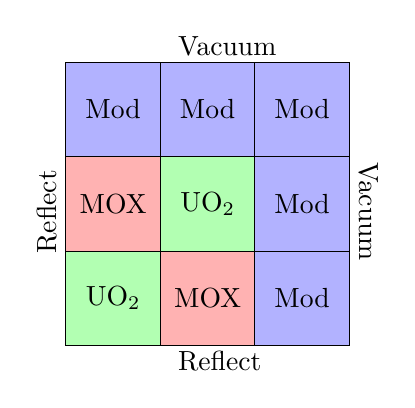
\begin{tikzpicture}[scale=0.4, every node/.style={scale=1}]
        \filldraw[xshift=6 cm, yshift=0 cm, fill=blue!30!white, draw=black] 
        (0, 0) rectangle (3,3) node[pos=.5] {Mod};
        \filldraw[xshift=6 cm, yshift=3 cm, fill=blue!30!white, draw=black] 
        (0, 0) rectangle (3,3) node[pos=.5] {Mod};
        \filldraw[xshift=6 cm, yshift=6 cm, fill=blue!30!white, draw=black] 
        (0, 0) rectangle (3,3) node[pos=.5] {Mod};
        \filldraw[xshift=3 cm, yshift=6 cm, fill=blue!30!white, draw=black] 
        (0, 0) rectangle (3,3) node[pos=.5] {Mod};
        \filldraw[xshift=0 cm, yshift=6 cm, fill=blue!30!white, draw=black] 
        (0, 0) rectangle (3,3) node[pos=.5] {Mod};
        \filldraw[xshift=0 cm, yshift=0 cm, fill=green!30!white, draw=black] 
        (0, 0) rectangle (3,3) node[pos=.5] {UO$_2$};
        \filldraw[xshift=3 cm, yshift=3 cm, fill=green!30!white, draw=black] 
        (0, 0) rectangle (3,3) node[pos=.5] {UO$_2$};
        \filldraw[xshift=3 cm, yshift=0 cm, fill=red!30!white, draw=black] 
        (0, 0) rectangle (3,3) node[pos=.5] {MOX};
        \filldraw[xshift=0 cm, yshift=3 cm, fill=red!30!white, draw=black] 
        (0, 0) rectangle (3,3) node[pos=.5] {MOX};
        \draw[xshift=9cm,yshift=4.25cm] node[right] 
        {\rotatebox{-90}{Vacuum}};
        \draw[yshift=4.25cm] node[left] {\rotatebox{90}{Reflect}};
        \draw[xshift=3.25cm,yshift=9.5cm] node[right] {{Vacuum}};
        \draw[xshift=3.25cm, yshift=-.5cm] node[right] {{Reflect}};
    \end{tikzpicture}
\end{document}
